\begin{figure}
	\centering
	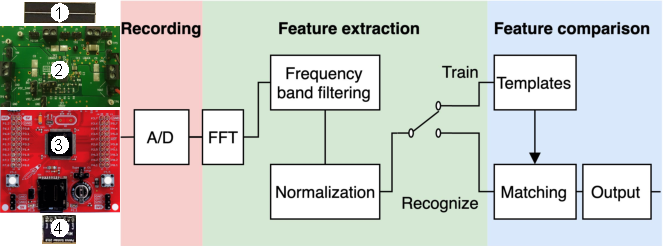
\includegraphics[width=\columnwidth]{figures/cis}
	\caption{\fullCIM: an instant of a \fullsys. \cim features a power failure immune word recognizer. Once a word is recorded, the word's spectral features extraction begins. The resulting features vector is compared against previously-stored words' templates for recognition. The comparison using a liner distance matching algorithm}
	\label{fig:cis}
\end{figure}

We have developed a prototype of a \fullcim (\cim): an instant of a \fullsys. The \cim consists of eight batteryless intermittent nodes. Each node is capable of performing isolated words recognition. 

The reason behind developing a \cim is threefold: (i) voice is a natural and convenient way for human to interact with miniaturized devices; (ii) demonstrating \textit{the world's first} batteryless intermittently-powered command recognizer, which shades light on the potential of batteryless intermittent systems; and (iii) facilitating testing with different sensing strategies and different type of external events arrival (i.e., regular  or burst). 


% Moreover, we believe that a \cim can facilitate direct human-to-human or human-to-objects communication. Imagine that a \cim based system is deployed in a play ground, embedded in ground and other objects. You want to call your child, and a \cim based system is embedded in your shirt and his shirt. You say his name and the \cim picks up the word and scatter it over light---\cite{marco}  demonstrates the feasibility of scattering sunlight to communicate between two nodes that are up to 60\,m apart. The scattered signal will be relied on other \cim nodes until the receiving node on his shirt receives the message and notify him, daddy is calling. 

\subsection{Hardware}
\label{sec:hardware}
A \cim node consists of thee main parts: a microphone, a microcontroller, and a harvester. MSP430RF5994~\cite{ti_msp430_website}, an ultra-low-power microcontroller, is used for data acquisition and processing. This microcontroller has a 16-bit RISC processor running on 1 MHz, 8KB of SRAM (volatile), 256KB of FRAM (non-volatile), and a 12-bit analog to digital converter (ADC). It also features a Low Energy Accelerator (LEA), which offloads the main CPU for specific operations, such as FFT. For recording we use the PMM-3738-VM1010-R piezoelectric MEMS microphone, which features Wake on Sound and ZeroPower listening technologies \cite{microphone}, allowing both the microcontroller and the microphone to sleep in a low-power mode until a sound wave is detected.
The microcontroller and microphone are powered by a BQ25570 solar power harvester~\cite{BQ25570EVM-206_website} connected to an IXYS SLMD121H04L solar cell~\cite{SLMD121H04L_website} and a super-capacitor of 470 \si{\micro F}. For debugging we used the Saleae logic analyzer~\cite{saleae}.

\subsection{System Description}
The \cim has a power interrupts immune command recognizer. The recognizer is capable of recognizing isolated-word type of speech. 
The main parts of the recognizer are illustrated in Figure~\ref{fig:cis} and explained below:

\subsubsection{Data acquisition}
The \textit{Wake-on-Sound} feature of the microphone triggers the data acquisition process once the energy level in the sound signal crosses a certain level. The ADC, then, samples the output of the microphone at 8\,kHz. This sampling rate is sufficient to cover most of the frequency range of the human voice. To determine the end of the recording we relied on the characteristics of the targeted vocabulary. In particular, we identified experimentally the minimum effective recording length, which is 
%happened be 
285\,ms for the chosen set of words. By exploiting the Wake-on-Sound feature and using the minimum effective recording length, we eliminate the need for an endpoint detection algorithm, greatly improving the processing time and system efficiency from the energy perspective.


\subsubsection{Feature Extraction}
Once a recording has finished, framing and data processing begin. \cim divides the digitized signal into non-overlapping frames of 256 samples ($\approx$ 33 milliseconds). This size is beneficial for doing a Fast Fourier Transform and short enough for the voice-features to be considered constant inside a frame.

To extract the spectral features of a frame, \cim divides the frequency of interest into 12 bands (as in~\cite{hopper1992}). The first five bands has a bandwidth of 200\,Hz. The next three has a bandwidth of 300\,Hz which is followed by two bands of 500\,Hz. Finally, the last two bands has a 600\,Hz bandwidth. This division is motivated by how the energy is concentrated in human speech~\cite{hopper1992}. Then, \cim computes the 256-point Fast Fourier Transform for each frame. The resulting feature vector contains the amount of energy concentrated in each frequency band defined earlier. This feature vector forms the basis for the words identifying process once it is normalized.

We normalize the feature vectors to minimize detection errors that result from differences in the amplitude of the speech input. To normalize a feature vector, \cim computes the binary logarithm of each entry of that vector. 
Then it computes the mean of the resulting vector. Finally, it subtracts the computed mean from each entry of the resulting vector. This is summarized in the following equation: 
\begin{equation}
    f_i = \log(\hat{f}_i) - \frac{\sum\limits^S_{i=1}\log(\hat{f}_i)}{S},
\end{equation}
where $f_i$ is the normalized output for the $i^{\text{\tiny th}}$ spectral band of a feature vector, $\hat{f}_i$ is the energy in the $i^{\text{\tiny th}}$ spectral band of the frame, and $S$ is the number of spectral bands (12 in our case). 

\subsubsection{Feature Matching}
% %
% \begin{figure}
% \centering
% 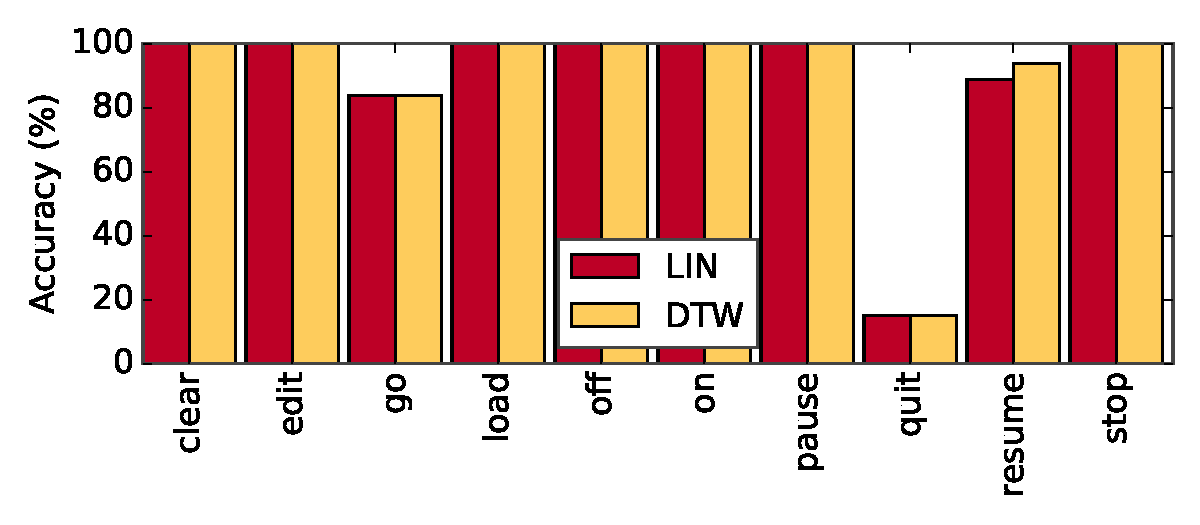
\includegraphics[width=\linewidth]{figures/DTWvsLDM}
% \caption{Recognition accuracy for linear matching and DTW when using 9 frames as the recording length.}
% \label{fig:DTWvsLDM}
% \end{figure}
% %
\begin{table}
	\centering
	\caption{Profiling of features matching algorithms: Dynamic Time Warping (DTW) and Linear Distance Matching (LDM)}
	\label{tab:profiling}
	\begin{tabular}{lll} \hline
	Section & LDM (ms) & DTW (ms) \\\hline
	Recording & 285  & 285 \\
	Feature extraction & 501 & 501 \\
	Feature matching &  99 & 1251 \\\hline
	Total & 885 & 2037 \\\hline
	\end{tabular}
\end{table}
%
Feature matching is achieved by computing the distances between the normalized feature vectors of the recorded word and the feature vectors of the words stored during the training phase (templates). 
\cim computes the squared Euclidean distance between vectors as follows:
\begin{equation}
	 	d_j = \sum\limits^S_{i=1} (f_{s,i} - f_{r,i})^2,
    \label{eq:frame_dist}
\end{equation}
where $d_j$ is the distance between the $j^{\text{\tiny th}}$ stored and recorded vectors. $f_{s,i}$ is the normalized output of the $i^{\text{\tiny th}}$ spectral band of a stored vector, $f_{r,i}$ is the normalized output of the $i^{\text{\tiny th}}$ spectral band of a recorded vector. 
The total distance between two words is calculated as follows:
\begin{equation}
		D_k = \sum\limits^{l}_{j=1} d(j)
\end{equation}
where $D_k$ is the distance between the $k^{\text{\tiny th}}$ stored word and the recorded word, and $l$ is the recording length measured in frames.

Once the recorded word has been compared to all \cim template words, the template with the smallest distance to the recorded word is considered the correct word. However, if the smallest distance is bigger the garbage threshold which we experimentally set, then the \cim will return "undefined word". 

It should be emphasized that in linear distance matching (LDM) the feature vectors of two words are compared successively, not accounting for differences in pronunciation speed. This is sufficient for our case as we are targeting isolated words and speaker dependent speech recognition type. We also implemented the Dynamic Time Warping algorithm which better handles the difference in the speed of speech. However, it is slower than the linear matching algorithm  (Table~\ref{tab:profiling}) and the detection accuracy was comparable in our case.% (Figure~\ref{fig:DTWvsLDM}). 

\subsubsection{Power Failure Protection}
In order to preserve the progress state and to protect \cim data against randomly timed power failures, we manually split \cim program into 19 atomic regions. We ensured the each of these regions requires less energy then what the energy buffer can provide with a single charge. The program progress state is saved in the non-volatile memory (FRAM) on the transition between these regions. This prevents the program from falling back to its starting point (\texttt{main()}) after each power failure. Data in the non-volatile memory with Write-After-Read dependency is double buffered to ensure data integrity when the power supply is interrupted. 

\subsection{Code profiling}
The entire command recognition software was written in the {\tt C} programming language. The total program consists of 973 lines of code, excluding the FFT function from the Texas Instrument DSP library. See Table~\ref{tab:code_stats} for more information.

The memory footprint on the microcontroller is 20,064 bytes of FRAM and 1,134 bytes of SRAM. Execution times are shown in Table~\ref{tab:profiling}.

The power usage of a node differs according to it's activity. When a node is waiting for a voice event, it is in low-power mode. When data needs to be processed or recorded it is in active mode. When recording, the microphone and ADC consume additional power. The power consumption rates are determined by measuring the current with a Monsoon power monitor~\cite{monsoon} and shown in Table~\ref{tab:power_usage}.


\begin{table}
	\centering
	\caption{Code statistics: lines of code}
	\label{tab:code_stats}
	%Compiled without optimization flags:
	\begin{tabular}{lrrrr} \hline
		Language & Files & Blank & Comment & Code \\\hline
		C & 7 & 264 & 173 & 736 \\
		C/C++ Header & 8 & 62 & 40 & 237 \\\hline
		Total &  15 & 326 & 213 & 973 \\\hline
	\end{tabular}
\end{table}

\begin{table}
	\centering
	\caption{Power usage.}
	\label{tab:power_usage}
	%Compiled without optimization flags:
	\begin{tabular}{lrrr}\hline
	Section & Current (\si{\micro A}) & Voltage (V) &  Power (\si{\micro W}) \\\hline
	Sleeping & 64 $\pm$20 & 2.008 & 128 $\pm$40 \\
	Recording & 423 $\pm$20  & 2.008 &  849 $\pm$40\\
	Processing &  282 $\pm$20 & 2.008& 566 $\pm$40 \\\hline
	\end{tabular}
\end{table}